\documentclass[a4paper, 11pt, titlepage]{article}
\usepackage{hyperref}
\usepackage{fancyhdr}
\usepackage{graphicx}
\usepackage{subcaption}
\usepackage{imakeidx}
\usepackage{makeidx}
\usepackage{mathtools}
\usepackage[spanish]{babel}
\usepackage{eurosym}

\setcounter{secnumdepth}{5}
\setcounter{tocdepth}{5}

% Variables
\title{{\scshape\Huge Infraestructura de Redes Privadas Virtuales (VPN) \par}}
\author{Francisco Javier Balón Aguilar}
\date{enero de 2019}

% -------------------------------------------------------------------------------------------------------------------------------------

\begin{document}
\maketitle
\renewcommand{\contentsname}{Índice}
\tableofcontents
% \newpage
%Lista de figuras 
\listoffigures
%\newpage

%Lista de tablas 
%\listoftables
\newpage

\section{Breve contextualización histórica y teórica de redes e infraestructuras VPN}

    Como de cosumbre me gusta iniciar cualquier contextualización con un breve histórico del
    tema a tratar. En el caso de las \textit{redes privada virtuales}, o \textit{VPN} 
    (\textit{virtual private network}, en inglés) como se acostumbran a llamar hay poco que
    decir; algunos expertos atribuyen la creación de esta tecnología de redes informáticas a
    \textit{Gurdeep Singh-Pall}, vicepresidente de \textit{Microsoft}. 

    \textit{Singh-Pall} desarrolló entre 1995 y 1996 los protocolos \textit{PPTP} o \textit{
    Point-to-Point Tunneling Protocol}, tecnología que permitía la creación de túneles lógicos
    entre máquinas de la misma forma que si hubiera un cable físico de red entre ellas. Nacieron
    así las consideradas primeras \textit{VPN}. En los primeros años estas redes tenían un uso escaso 
    y puntual, utilizado por algunas empresas y gobiernos para compartir redes (y con ellas información) 
    de forma segura y privada; aunque el protocolo \textit{PPTP} hoy en día se considera obsoleto e 
    inseguro. Ya no se recomienda su uso a no ser que la confidencialidad, disponibilidad e integridad de
    la información no sea necesaria. \textit{PPTP} presenta una ventaja ofreciendo altas tasas de 
    transferencia de datos y una fácil y rápida configuración e implementación, pero pierde si las 
    contraponemos a sus desventajas en seguridad.
    
    El protocolo \textit{L2F(Layer 2 Forwarding)} se creó en las primeras etapas del desarrollo de las VPN.
    Como \textit{PPTP}, \textit{L2F} fue diseñado por \textit{Cisco} para establecer túneles de tráfico desde 
    usuarios remotos hasta sus sedes corporativas. La principal diferencia entre \textit{PPTP} y \textit{L2F} 
    es que, como el establecimiento de túneles de L2F no depende del protocolo IP, es capaz de trabajar directamente
    con otros medios y protocolos. L2F también difiere de PPTP en que permite que los túneles contengan más 
    de una conexión. 

    El desarrollo y los avances hizo que estas formas mutara y diera lugar a otros protocolos, dando 
    distintos tipos de \textit{VPN}, mejorando principalmente los algoritmos de cifrados y la 
    seguridad de las mismas (motivados por los riesgos y amenazas que han ido creciendo, de forma 
    exponencial conforme la tecnología se ha ido desarrollando). 

    Aproximadamente en 1999 surgió un protocolo como mejora de tanto \textit{LF2} como \textit{PPTP}, al 
    que denominaron \textit{L2TP}. Este protocolo no ofrece criptografía o autenticación fuerte por sí 
    mismo, por lo que se combina con el protocolo \textit{IPsec} para suplir estas características de 
    seguridad. Podemos decir que a partir de este momento la seguridad se convirtió en algo primordial
    en lo que protocolos VPN se refiere, Microsoft desarrolló posteriormente \textit{IKEv2} (desarrollado 
    en conjunto con Cisco, también se puede combinar con \textit{IPsec} para lograr un potente cifrado, 
    dando lugar a \textit{IKEc2/IPsec}) y \textit{SSTP} (que utiliza cifrado SSL 3.0 altamente seguro).

    \textit{James Yonan} estaba viajando por Asia Central en los días previos al 11 de septiembre de 2001 y conectándose
    a su oficina a través de Proveedores de Internet asiáticos o rusos. El hecho de que estas conexiones se 
    establecieran a través de servidores en países con una seguridad dudosa lo hizo cada vez más consciente y 
    preocupado por estos problemas. Su investigación reveló que había dos corrientes principales en la tecnología
    VPN, una promoción de la \textbf{seguridad}, y la otra \textbf{usabilidad}. Ninguna de las soluciones disponibles
    (expuestas anteriormente) en ese momento ofrecía una mezcla ideal de ambos objetivos. \textit{IPsec} y sus 
    implementaciones eran difíciles de establecer, pero ofrecían una seguridad aceptable. Sin embargo, su compleja
    estructura lo hacía vulnerable a ataques, errores y fallos de seguridad. Por lo tanto, el enfoque de red que 
    \textit{Yonan} encontró en algunas de las soluciones del campo de usabilidad pareció tener más sentido para él, 
    llevándolo a un modelo de red modular usando los dispositivos de red virtuales \textit{TUN/TAP} que son proporcionados 
    por el núcleo Linux (esto lo veremos en profundidad más adelante).

    La elección de los dispositivos \textit{TUN/TAP} como modelo de red ofreció inmediatamente una flexibilidad que otras 
    soluciones VPN no podían ofrecer, utilizando este potencial y las librerías abiertas de \textit{OpenSSL} denominó a 
    su tecnología \textit{OpenVPN}, también software libre (bajo licencia GPL) y de código abierto. \textbf{\textit{OpenVPN} es 
    considerado el mejor, más felixble y más seguro protocolo de VPN hasta la fecha.} El potencial de su código C abierto
    permite un crecimiento y una adaptación antes no vista; permite autenticación por pares de claves compartidas, cuentas
    de usuario, certificados; puede correr sobre prácticamente cualquier sistema operativo, etc.

    \subsection{Usos generales, usos prácticos en comunicaciónes, privacidad \& seguridad}

        Hoy en día podemos diferenciar las redes privadas virtuales en dos grupos dependiendo de la finalidad de su
        uso:
        
        \begin{enumerate}
            \item \textit{Redes VPN comerciales}. Se trata de empresas u organizaciones que ofrecen a los usuarios el
            servicio de una red privada virtual especializada, dando al usuario una o varias direcciones aisladas dentro 
            de su propia red con el fin de dotar a éste de los beneficios de esta tecnología. 
            
            Esto es usado por los usurios con diversos fines, siendo los más comunes:
        
            \begin{itemize}
                \item La capa extra de seguridad en la transmisión de datos que ofrece la criptografía empleada por el 
                servicio, ofreciendo criptografía -al menos hasta el servidor- en paquetes que por defecto no llevan, 
                como páginas web sin cifrar (\textit{HTTP}) o comunicaciones no seguras (\textit{telnet}) y añade una segunda
                capa de cifrado a los protocolos y servicios ya cifrados. Esto es 
                interesante si solemos frecuentar redes públicas de las que queremos una capa de abstracción y 
                <<acorazamiento>> de nuestros paquetes evitando atacantes en estas redes.
                \item Relacionado con lo anterior, esta criptografía mejora la privacidad y/o el anonimato del usuario
                que opera en la red, evitando miradas y escuchas indiscretas en sus comunicaciones por medio de las capas
                de cifrado extra que encapsulan los paquetes de red. Un ejemplo práctico de ello son los espías occidentales
                en países como China, con un altísimo grado de espionaje gubernamental. Lo que obliga a estos agentes a 
                utilizar redes VPN con servidores fuera del dominio -siguiendo con el ejemplo- chino de forma que no puedan,
                al menos fácilmente, espiar sus comunicaciones.
                \item Un uso también de moda hoy día supone el salto virtual geográfico. Al utilizar redes VPN nuestra salida
                a la red no sería el router al que estamos conectados físicamente (entendiendo físicamente las ondas 
                electromagnéticas de la tecnología Wi-Fi o cualquier tecnología inalámbrica) sino el servidor VPN del que somos 
                clientes. Esto implica que, a los ojos de servicios de red a los que nos conectamos, <<estamos>> donde nuestro
                servidor. 
                Con la popularidad de servicios de Streaming como Netflix o Amazon Prime Video que restringen geográficamente
                el contenido (es común escuchar que una obra cinematográfica sale, a veces, meses antes en Estados Unidos que
                en el resto del mundo) se ha popularizado el uso de estas redes pretendiendo engañar al servicio y hacerle pensar
                que somos un usuario de una u otra geolocalización \footnote{Cabe destacar que esto es a veces problemático cuando
                utilizamos dispositivos móviles, que son altamente geolocalizables mediante otros métodos como la triangulación de 
                datos, las redes Wi-Fi conectadas, el GPS incorporado, etc.}.
                \item Y también relacionado con lo anterior, la búsqueda de saltar otro tipo de restricciones de los proveedores de
                Internet (\textit{ISP}) como restricciones a descargas \textit{P2P} o puertos específicos de algunos juegos o 
                servicios particulares.
            \end{itemize}

            \item \textit{Infraestructuras VPN}. Estas no están destinadas al público común ni abiertas, más bien todo lo contrario.
            Las infraestructuras de este tipo se diseñan e implementan con un objetivo concreto y buscando, como bien indicó 
            \textit{James Yonan}:
            
            \begin{itemize}
                \item \textit{Seguridad.} Garantizando la integridad, confidencialidad y disponibilidad tanto de las comunicaciones 
                como de los servicios.
                \item \textit{Usabilidad.} Extendiendo la red para saltar las barreras físicas y permitir comunicaciones LAN sin 
                importar hardware de red o geolocalización de los nodos que la componen, ahorrando costes y permitiendo dar forma
                virtual y robustez a una infraestructura de red propia.
            \end{itemize}

        \end{enumerate}

    \section{Consideraciones previas}

        Una vez introducido y contextualizado, en el presente documento buscamos la implementación de
        una \textbf{infraestructura VPN no comercial}, basada en el procotolo seguro, abierto y altamente
        configurable y escalable de \textit{James Yonan}: \textbf{OpenVPN}, con los objetivos de lograr
        la seguridad y usabilidad que el protocolo ofrece, poniendo especial énfasis en la seguridad y
        la defensa del sistema, por lo que se detallarán procesos de \textit{hardening} tanto de los 
        sistemas como de las redes.

    \subsection{Servidor OpenVPN}

        El \textbf{servidor} OpenVPN es el servidor central de la infraestructura y el más alto en la 
        jerarquía de servidores de la misma. Es éste el encargado crear el servicio VPN que vamos a 
        implementar para gestionar las comunicaciones de los clientes y la estabilidad de la red.

        Con la vista puesta en ello, se utilizará como \textbf{servidor} un VPS\footnote{
            \textit{VPS, Virtual Private Server ó Servidor Privado Virtual} es una partición virtual dentro 
            de un servidor físico que le asigna recursos exclusivos a cada partición. Éstas otorgan acceso 
            raíz que permite instalar un sistema operativo y trabajar con alto grado de libertad.
        } con el sistema GNU/Linux en su distribución Arch Linux.

        \paragraph{¿Por qué VPS?} La elección de la tecnología VPS para su utilización como servidor 
        atiende a las razones de ahorro de costes y simplicidad, delegando el mantenimiento físico y 
        hardware al proveedor y mejorando así tanto la disponibilidad del servicio como el rendimiento 
        y escalabilidad del servidor.

        Una segunda opción que ha sido barajada es la utilización de un servidor doméstico o privado
        conectado a cualquier red LAN de nuestra propiedad, como la de nuestra propia casa o empresa; 
        siendo esta segunda la opción más viable pero, debido a que estamos realizando una infraestructura
        VPN a nivel doméstico y académico la obviaremos.

        Una gran desventaja de la utilización de un servidor doméstico es la accesibilidad del mismo, ya
        que para hacerlo accesible mediante la red necesitaríamos que nuestro proveedor nos ofreciese una IP
        pública fija, en caso de ser una dirección dinámica, existe una opción interesante denominada 
        \href{https://www.noip.com/}{No-IP}\footnote{No-Ip es un servicio de DNS dinámico que traduce automáticamente un nombre de dominio dado y 
        fijo a la dirección pública que tenga nuestro equipo en cada momento, de forma que conociendo el nombre de dominio podemos 
        abstraernos a la dirección IP cambiante} y abrir los puertos necesarios en nuestro router, así como configurar el forwarding 
        entre el router y el servicio del servidor. Esto llevaría un trabajo extra de configuración y haríamos accesible nuestro router 
        doméstico, lo que lo haría susceptible a atacantes. Esto no es algo deseado ya que en esa misma red LAN tendríamos conectados otros 
        dispositivos personales, a menudo de otros familiares o compañeros, por lo que no es una idea viable para este caso.

        \paragraph{¿Por qué GNU/Linux?} La elección del sistema de Linus Torvalds atiende a innumerables
        razones que lo hacen el rey indiscutible en este campo:

        \begin{enumerate}
            \item \textbf{Estabilidad}. 
            \item \textbf{Seguridad}. 
            \item \textbf{Escalabilidad}. 
            \item \textbf{Flexibilidad}. 
            \item \textbf{Bajo coste económico}. 
            \item \textbf{Comunidad}. 
            \item \textbf{Libertad}. 
        \end{enumerate}

        Dentro del ecosistema GNU/Linux hemos elegido Arch Linux debido a que es uno de los <<sabores>> de 
        GNU/Linux más estables, robustos y seguros; además de ofrecer un sistema basado en la filosofía 
        KISS\footnote{\textit{Keep It Simple, Stupid!}} que permite que el sistema se adapte absolutamente
        a las necesidades del administrador/usuario, lo que permite adaptarnos a los recursos limitados del
        servidor VPS.

    \subsection{Servidor CA}

        El servidor CA o se compondrá de un servidor doméstico corriendo sobre en la distribución Arch Linux, al igual
        que el servidor VPN. Esto dotará al sistema de cohesión intrasistemas y dará robustez a la red.

    \subsection{Cliente \textit{terminator} servidor}

        Aunque puede resultar un poco confuso, este será el primer cliente de la red VPN y, por lo tanto,
        del servidor VPN. Este cliente será a su vez un servidor dedicado con diversos servicios que veremos
        en apartados posteriores.

        Se trata de un servidor doméstico corriendo, de nuevo, sobre la distribución Arch Linux para mantener
        la cohesión y consistencia de la red. El resto de clientes, lógicamente, serán contemplados
        como clientes multiplataforma, que veremos posteriormente tendrán diferentes y variados sistemas
        operativos.

\section{Implementación del servidor VPN}

    \subsection{Comprobación de soporte TUN/TAP}
    
        Antes de realizar estas comprobaciones es necesario tener claros unos conceptos teóricos referentes a las interfaces de redes 
        virtuales TUN y TAP, interfaces de red virtuales a nivel de kernel.
        
        \begin{figure}[htp]
            \centering
            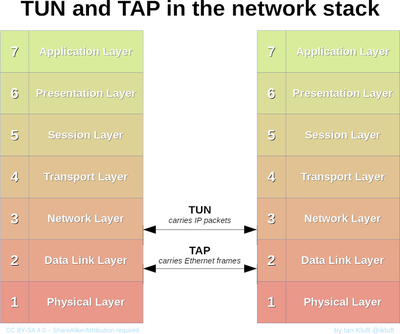
\includegraphics[width=0.6\textwidth]{resources/tuntap01.png}
            \caption{TUN y TAP en el modelo de capas OSI.}
            \label{fig:tuntap01}
        \end{figure}
    
        Aunque TUN y TAP tienen el mismo propósito de <<tunneling>> divergen en su funcionamiento técnico. Como vemos en la figura 
        \ref{fig:tuntap01}, TUN simula un dispositivo de capa de red y opera en la capa 3 del modelo OSI transportando paquetes IP mientras
        que TAP simula un dispositivo en la capa de enlace y opera en la capa 2 del modelo OSI, creando un puente (bridge) de red.
    
        Los paquetes enviados por un sistema operativo a través de un dispositivo TUN/TAP son entregados a un programa de espacio de usuario
        que se conecta al dispositivo. Un programa de espacio de usuario también puede pasar paquetes en un dispositivo TUN/TAP. En este caso 
        el dispositivo TUN/TAP inyecta estos paquetes a la pila de red del sistema operativo simulando así su recepción desde una fuente externa.
    
        \begin{figure}[htp]
            \centering
            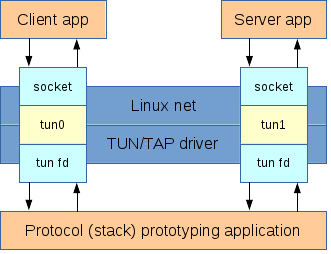
\includegraphics[width=0.6\textwidth]{resources/tuntap02.png}
            \caption{Diagrama que muestra el uso típico de los túneles TUN/TAP.}
            \label{tuntap02}
        \end{figure}
    
        En el caso de sistemas GNU/Linux, el soporte a TUN puede habilitarse de forma nativa en el kernel de Linux desde la versión 2.1.60\footnote{Véase:
        \href{https://github.com/torvalds/linux/blob/master/Documentation/networking/tuntap.txt}{github.com/torvalds/linux/blob/master/Documentation/networking/tuntap.txt}.
        Documentación oficial del kernel alojado en el repositorio de linux de su creador Linus Torvalds}. Debemos pues, comprobar si el kernel de nuestro
        servidor tiene habilitado éste soporte, ya que al utilizar un servicio VPS algunas capas de virtualización vServers y OpenVZ requieren que TUN
        esté habilitado en la máquina host y podría ser necesario contactar con el administrador o proveedor del servicio para ser habilitado y así poder 
        continuar. Debemos asegurar pues que el módulo CONFIG\_TUN está habilitado en el kernel, esto lo podemos ver rápidamente con la siguiente línea de 
        comandos:
        
        \begin{figure}[htp]
            \centering
            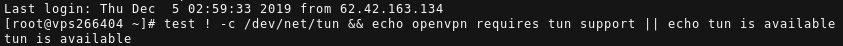
\includegraphics[width=1\textwidth]{resources/openvpn01.png}
            \caption{Salida de comando que demuestra el soporte TUN en nuestro kernel.}
            \label{tuntap02}
        \end{figure}
        
        Como podemos ver, nuestro servidor tiene el soporte para TUN habilitado, por lo que podemos continuar con normalidad; más tarde en la implementación
        veremos claramente el funcionamiento de estas interfaces de red, podemos proceder entonces con la instalación del servidor (software) VPN (OpenVPN).
    
        Debido a que nos encontramos utilizando la distribución Arch Linux, el sistema gestor de paquetes que utilizaremos será el propio de esta distribución, 
        denominado Pacman. La instalación es muy sencilla, simplemente usaremos el comando \textit{pacman -S openvpn} y el propio sistema se encargará de buscarlo
        en sus repositorios, descargarlo, descomprimirlo y compilarlo, ahorrando al usuario gran parte del trabajo.
        
        \begin{figure}[htp]
            \centering
            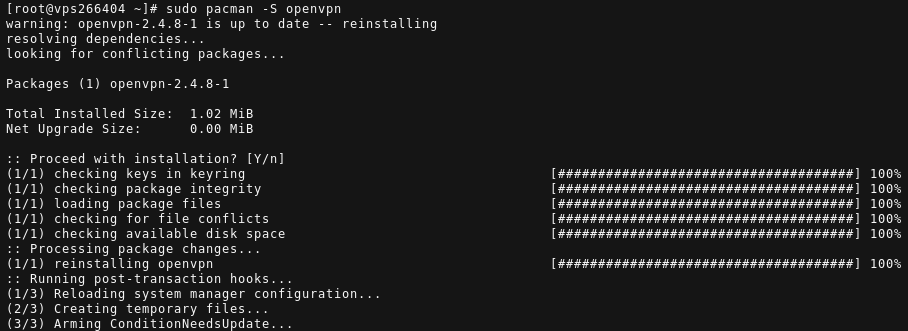
\includegraphics[width=1\textwidth]{resources/openvpn02.png}
            \caption{Instalación de \textit{openvpn} mediante \textit{pacman} en \textit{Arch Linux}.}
            \label{tuntap02}
        \end{figure}
        
        Este paquete trae consigo tanto el software necesario para levantar y configurar el servidor VPN como para configurar el cliente. El directorio 
        principal de OpenVPN es \textit{/etc/openvpn}, y en el mismo y será en este donde configuremos tanto nuestro servidor en este equipo, como la configuración
        de cada cliente en cada equipo remoto.
        
        \begin{figure}[htp]
            \centering
            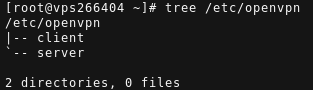
\includegraphics[width=0.5\textwidth]{resources/openvpn03.png}
            \caption{Contenido del directorio \textit{/etc/openvpn/}.}
            \label{tuntap02}
        \end{figure}

    \subsection{Implementación del servidor CA (Certificate Authority)}

        Cuando se levanta un servidor de OpenVPN es necesario crear un infraestructura de clave pública o PKI (Public Key Infrastructures, en inglés). Se trata de un 
        sistema informático (que engloba hardware, software, políticas y procedimientos de seguridad y criptografía asimétrica) que permite la ejecución de operaciones
        criptográficas como el cifrado, la firma digital y el no repudio de transacciones electrónicas.

        \begin{figure}[htp]
            \centering
            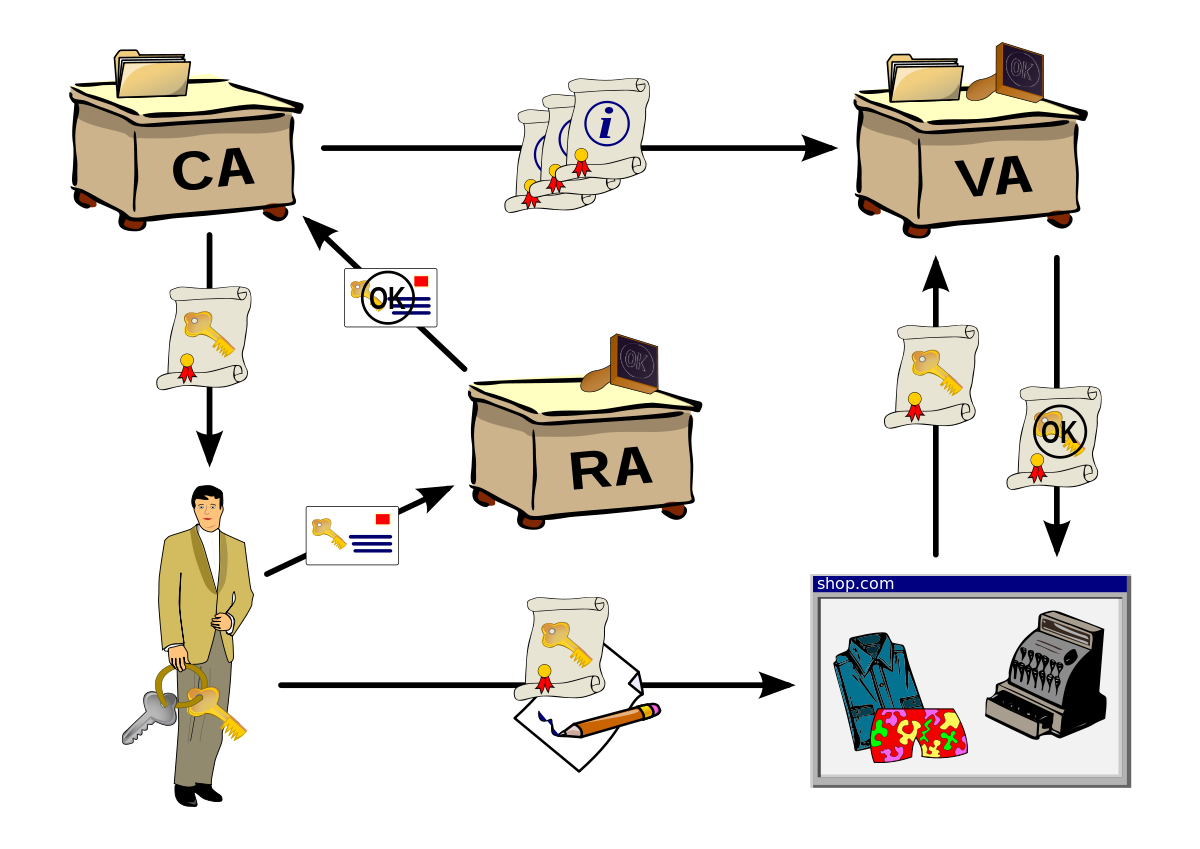
\includegraphics[width=0.6\textwidth]{resources/ca01.png}
            \caption{Diagrama que muestra la infraestructura de clave pública o PKI, siendo CA (Autoridad de Certificación), VA (Autoridad de Validación) y RA (Autoridad de
            Registro).}
            \label{tuntap02}
        \end{figure}

        En relación al servidor VPN, la creación del PKI consiste en:

        \begin{itemize}
            \item Creación de CA (Autoridad de Certificación - Certificate Authority) pública, seguido de su clave privada (PK).
            \item Un par de claves (una clave pública y una privada) para cada servidor, en nuestro caso nuestro servidor VPS Arch Linux.
            \item Un par de claves (una clave pública y una privada) para cada cliente.
        \end{itemize}

        El proceso es parecido a la autenticación basada en claves asimétricas utilizado en las comunicaciones SSH que trabajan con la capa añadida de CA. OpenVPN autentica 
        bidireccionalmente, por lo que el cliente debe autenticar el certificado del servidor y en paralelo, el servidor debe autenticar el certificado del cliente. 
        Esto se logra por la firma del tercero (la CA) en los certificados del cliente y del servidor. Una vez establecido esto, se realizan más controles antes de completar
        la autenticación que, de momento, se escapa a la propia competencia del PKI, por lo que no ahondaremos en ellos en este apartado. 

        \begin{figure}[htp]
            \centering
            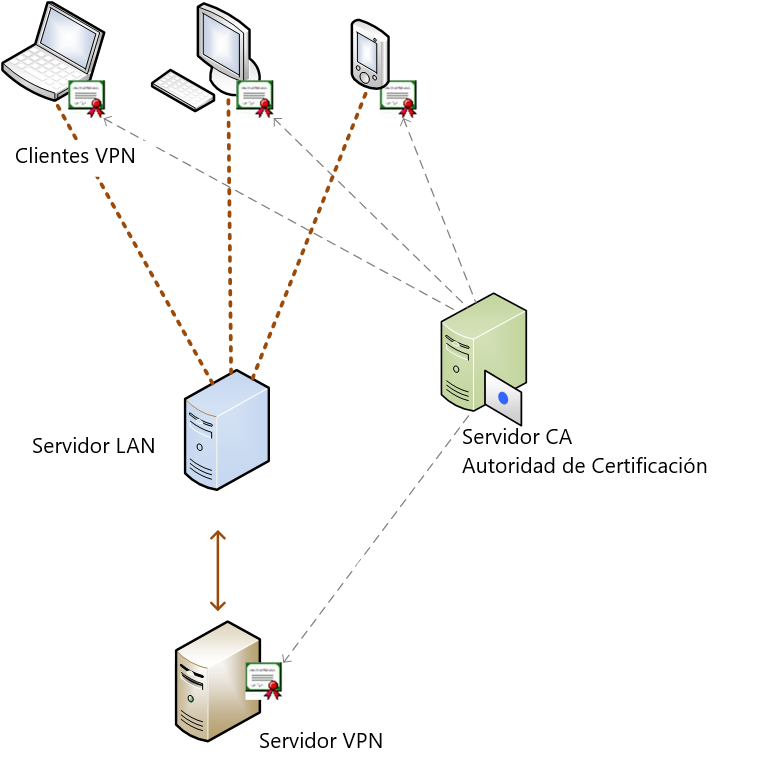
\includegraphics[width=0.6\textwidth]{resources/ca02.png}
            \caption{Diagrama básico que muestra el uso del servidor VPN con el servidor CA para el tratamiento de clientes.}
            \label{tuntap02}
        \end{figure}

        Por motivos de seguridad, el servidor CA no estará alojado en el mismo servidor VPN, de forma que si un atacante o persona no autorizada tuviera control sobre el 
        servidor VPN no pudiera generar o revocar claves y viceversa; si un atacante tuviera control sobre el servidor CA no pudiera manipular el servidor para permitir
        accesos no autorizados en la red VPN. Cumpliendo de esta forma con medidas de seguridad pasiva y aumentando la garantía de la integridad de la red y sus componentes,
        la disponibilidad dividiendo en dos los servidores (de forma que si uno cae el otro continuase funcionando) y la confidencialidad.

        Como servidor CA utilizaremos un equipo aislado de la red VPN, que será un servidor Debian Raspbian alojado en la red LAN de mi hogar. Para la comunicación y el
        intercambio de claves entre servidor CA y servidor VPN se utilizarán los protocolos SSH y SCP.

        \subsubsection{Generación de PKI (Public Key Infrastructures)}

            Lo primero que debemos hacer en el servidor CA es instalar el paquete \textit{easy-rsa}, una utilidad simple para autoridades de certificación basada en shell. 
            Utilizaremos de nuevo la utilidad \textit{pacman} para ello:
        
            \begin{figure}[htp]
                \centering
                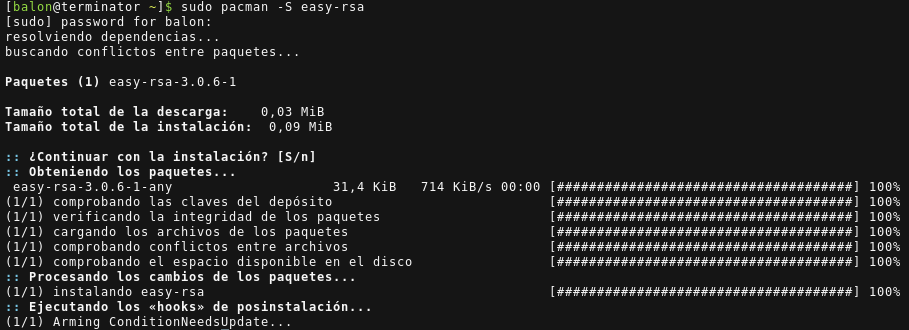
\includegraphics[width=1\textwidth]{resources/ca03.png}
                \caption{Instalación de \textit{easy-rsa} en servidor CA.}
                \label{ca03}
            \end{figure}
        
            \paragraph{Autoridad de Certificación (CA, Certificate Authority )}
        
            Para mejorar la seguridad y simplificar el sistema al mismo tiempo utilizaremos \textit{criptografía de curva elíptica}\footnote{
        
                En criptografía se habla de curva elíptica en referencia a una ecuación
                \[
                y^2=x^3+Ax+B
                \]
                que cumple $4A^3+27B^2\neq0$. Dando diferentes valores a $A$ y $B$
                obtenemos todo un conjunto de curvas que, al ser representadas, ofrecen 
                una forma similar. 
        
            } para las conexiones TLS. Para ello, tras la instalación
            de \textit{easy-rsa}, antes de cualquier generación y configuración añadiremos las siguientes líneas al archivo \textit{/etc/easy-rsa/vars}, lo que nos permitirá utilizar
            esta criptografía, dando más seguridad a las comunicaciones.
        
            \begin{figure}[htp]
                \centering
                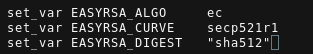
\includegraphics[width=0.5\textwidth]{resources/ca04.png}
                \caption{Apéndice añadido al fichero \textit{/etc/easy-rsa/vars}.}
                \label{ca04}
            \end{figure}
        
            Posteriormente levantaremos PKI y generamos el certificado CA del servidor.
        
            \begin{figure}[htp]
                \centering
                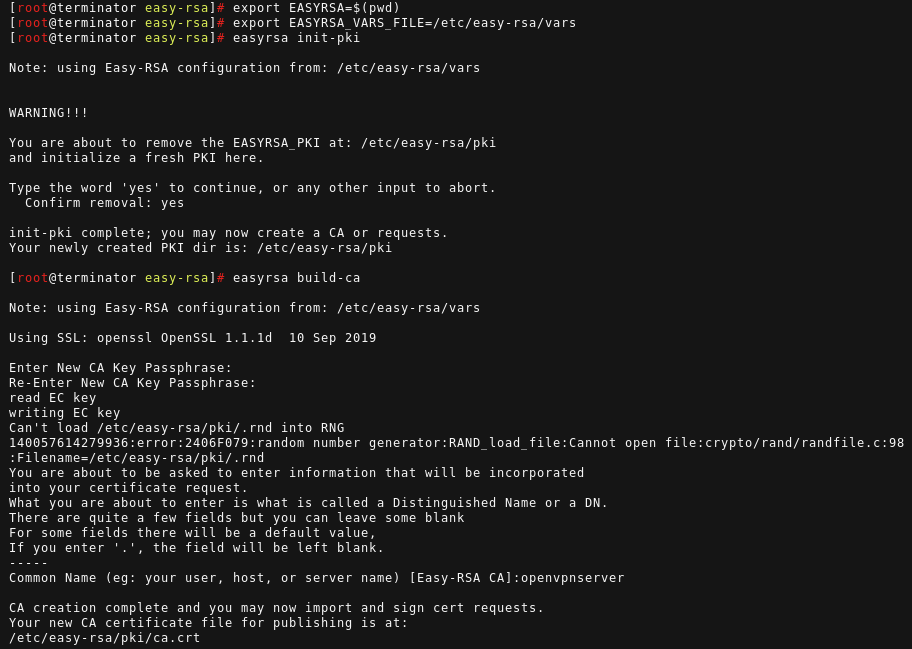
\includegraphics[width=1\textwidth]{resources/ca05.png}
                \caption{Levantamos PKI y generación de CA.}
                \label{ca05}
            \end{figure}
        
            \paragraph{Archivos del servidor VPN}
        
            Un servidor VPN funcional requiere de los siguientes elementos:
        
            \begin{itemize}
                \item Certificado público de autoridad de certificación (CA); ca.crt
                \item El archivo de parámetros de Diffie-Hellman\footnote{
        
                    El intercambio de claves de \textit{Diffie-Hellman} es un protocolo que permite un
                    intercambio secreto y seguro de claves entre dos partes que no han
                    tenido un contacto previo. Se usa ampliamente en criptografía y se basa
                    en el problema del logaritmo discreto (DLP), por lo que puede usarse
                    el mismo algoritmo a través del problema ECDLP.
                    
                    Al algoritmo puede resumirse en los siguientes pasos:
                    
                    \begin{enumerate}
                        \item Alice y Bob eligen una curva elíptica $E$ sobre un campo finito $Fq$ de
                        manera que el ECDLP sea computacionalmente difícil. También eligen un
                        punto $P$ en dicha curva de manera que su orden sea un número primo
                        grande.
                        \item Alice elige un entero grande $a$, calcula $PA=aP$ y envía $PA$ a Bob.
                        \item Bob elige un entero grande $b$, calcula $PB=bP$ y envía $PB$ a Alice.
                        \item Alice calcula $aPB=abP$
                        \item Bob calcula $bPA=abP$
        
                    \end{enumerate}
        
                    Al finalizar el algoritmo, tanto Alice como Bob disponen de $abP$. Pero un
                    usario que escuche el canal solo habrá podido obtener $PA$ y $PB$, los
                    cuales no le permiten calcular $abP$ a menos que resuelva el ECDLP. Alice
                    y Bob solo tendrán que extraer una clave a partir de abP y usarla para
                    enviar datos cifrados. Para tal propósito podrán usar cualquier
                    algoritmo simétrico como DES, AES, etc.
        
                } (DH), requerido por el modo TLS cuando \textbf{no} se utilizan curvas elítpicas, 
                no es el caso actual; dh.pem.
                \item El par de claves de servidor (clave pública y privada); servername.crt y servername.Key.
                \item El código de autenticación basado en Hash (HMAC); ta.key.
            \end{itemize}
        
            Por lo que al finalizar estos pasos el usuario habrá generado los siguientes archivos en el 
            servidor:
        
            \begin{itemize}
                \item \textit{/etc/openvpn/server/ca.crt}
                \item \textit{/etc/openvpn/server/servername.crt}
                \item \textit{/etc/openvpn/server/servername.key}
                \item \textit{/etc/openvpn/server/ta.key}
            \end{itemize}
        
            Comenzaremos enviando el certificado público de CA al servidor VPN, utilizando el protocolo SCP. 
            El servidor, al recibirlo lo moverá al directorio \textit{/etc/openvpn/server/}.
        
            \begin{figure}[htp]
            \centering
                \begin{subfigure}[b]{1\linewidth}
                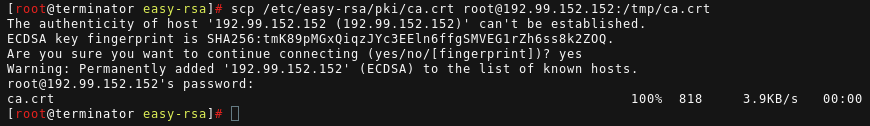
\includegraphics[width=1\textwidth]{resources/ca06.png}
                \caption{Envío mediante el protocolo \textit{SCP} del certificado \textit{ca.crt} al servidor VPN.}
                \end{subfigure}
            
                \begin{subfigure}[b]{0.7\linewidth}
                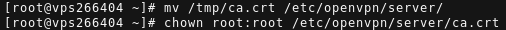
\includegraphics[width=1\textwidth]{resources/ca07.png}
                \caption{Obtención de \textit{CA} recibido por parte del servidor y movido a \textit{/etc/openvpn/server/}.}
                \end{subfigure}
            \caption{Intercambio de archivos.}
            \label{fig:ca0607}
            \end{figure}
        
            A continuación generaremos el par de claves del servidor. Esto lo haremos en el propio servidor,
            por lo que deberemos instalar el paquete \textit{easy-rsa} al igual que hicimos en el servidor CA.
        
            \begin{figure}[htp]
                \centering
                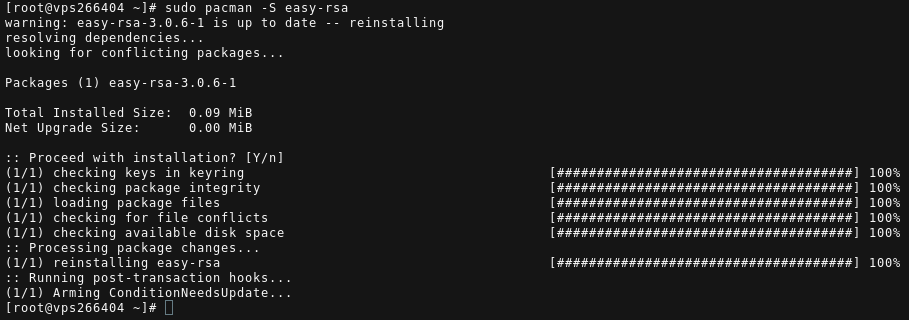
\includegraphics[width=1\textwidth]{resources/ca08.png}
                \caption{Instalación de \textit{easy-rsa} en el servidor VPN.}
                \label{ca08}
            \end{figure}
        
            Generamos entonces el par de claves mediante los siguientes comandos:
        
            \begin{figure}[htp]
            \centering
                \begin{subfigure}[b]{1\linewidth}
                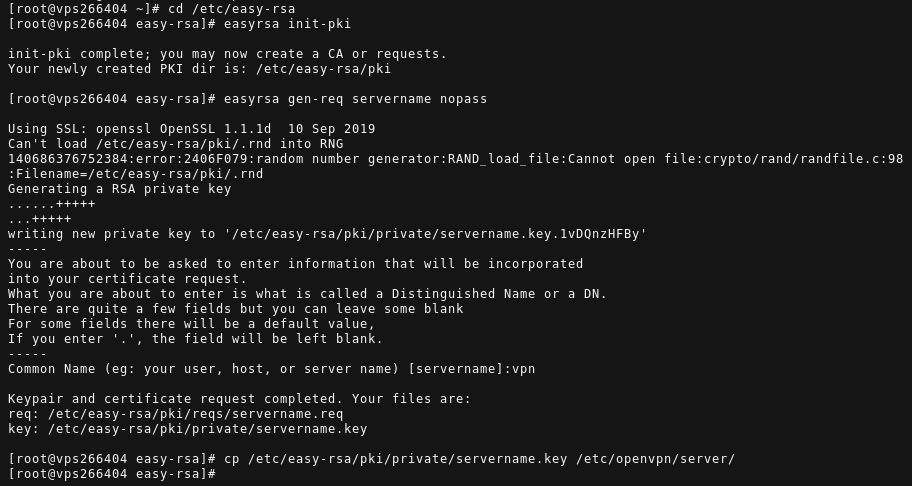
\includegraphics[width=1\textwidth]{resources/ca09.png}
                \caption{Generación de claves del servidor con \textit{easy-rsa}.}
                \end{subfigure}
            
                \begin{subfigure}[b]{0.7\linewidth}
                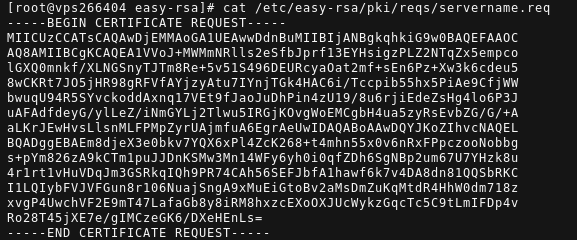
\includegraphics[width=1\textwidth]{resources/ca10.png}
                \caption{Clave pública del servidor.}
                \end{subfigure}
        
                \begin{subfigure}[b]{0.7\linewidth}
                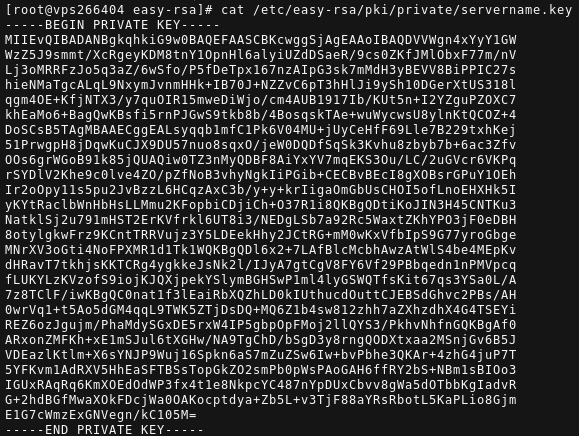
\includegraphics[width=1\textwidth]{resources/ca11.png}
                \caption{Clave privada del servidor.}
                \end{subfigure}
            \caption{Generación y firma de claves.}
            \label{fig:ca091011}
            \end{figure}
        
            Lo que nos dará como resultados los ficheros correspondientes a las claves RSA pública y privada,
            respectivamente (Figuras \ref{fig:ca091011}).
        
            \newpage
            Finalmente crearemos, también en el servidor VPN el código de autenticación basado en Hash (HMAC).
        
            Esto se usará para añadir una firma HMAC adicional a todos los paquetes handshake de SSL/TLS.
            Además cualquier paquete UDP que no tenga la firma HMAC correcta será inmediatamente desechado, 
            protegiendo contra:
        
            \begin{itemize}
                \item Portscanning.
                \item Ataques DOS contra el puerto UDP de OpenVPN.
                \item Iniciaciones SSL/TLS handshake de máquinas no autorizadas y robos de identidad.
                \item Cualquier vulnerabilidad eventual de desbordamiento de búfer en la implementación de SSL/TLS.
            \end{itemize}
        
            \begin{figure}[htp]
                \centering
                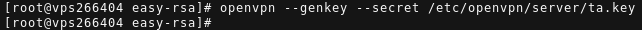
\includegraphics[width=1\textwidth]{resources/ca12.png}
                \caption{Generación de clave HMAC.}
                \label{ca12}
            \end{figure}
        
            \paragraph{Archivos de cliente VPN}
        
            Cualquier máquina puede generar sus propios archivos de cliente mientras \textit{easy-rsa} esté
            instalado. En nuestro caso hemos optado por un servidor al que hemos denominado \textit{terminator}:
        
            \begin{figure}[htp]
                \centering
                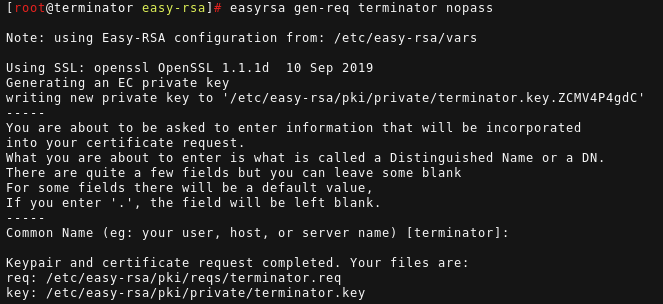
\includegraphics[width=1\textwidth]{resources/ca13.png}
                \caption{Generación de claves para el cliente \textit{terminator}.}
                \label{ca13}
            \end{figure}
        
            Esto habrá creado el par de claves como vemos:
        
            \begin{figure}[htp]
                \centering
                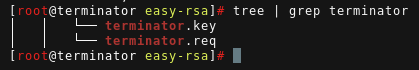
\includegraphics[width=0.7\textwidth]{resources/ca14.png}
                \caption{Par de claves de \textit{terminator}.}
                \label{ca14}
            \end{figure}
        
            Podemos realizar este paso como tantos clientes haya.
        
            \paragraph{Firma de certificados de servidor y cliente}
        
            Una vez hemos generado todos los archivos necesarios de cara al servidor y el cliente,
            sólo necesitamos enviarlos al servidor CA para que éste los firme y sean devueltos a sus
            respectivas máquinas, ya firmados.
        
            \begin{figure}[htp]
                \centering
                
\includegraphics[width=1\textwidth]{resources/ca15.png}
                \caption{En el servidor VPN preparamos la clave pública \textit{servername.req} para su
                recepción por el servidor CA moviéndolo a la carpeta temporal \textit{/tmp}.}
                \label{ca15}
            \end{figure}
            \begin{figure}[htp]
                \centering
                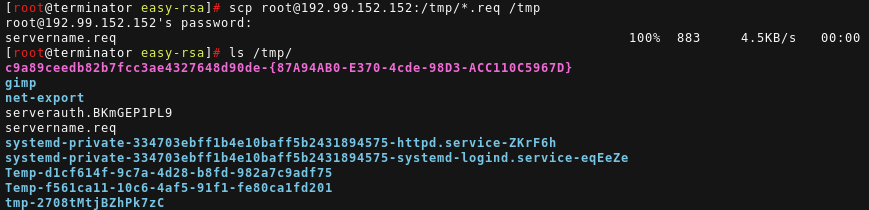
\includegraphics[width=1\textwidth]{resources/ca16.png}
                \caption{Recepcionamos en el servidor CA la clave pública del servidor.}
                \label{ca16}
            \end{figure}
        
            Una vez el servidor CA tenga las claves públicas necesarias (servidor y clientes, que en 
            nuestro caso sólo añadimos de momento uno: \textit{terminator}), las firmaremos.
        
            Es necesario indicar a \textit{easy-rsa} qué estamos firmando; en este caso el servidor:
        
            \begin{figure}[htp]
                \centering
                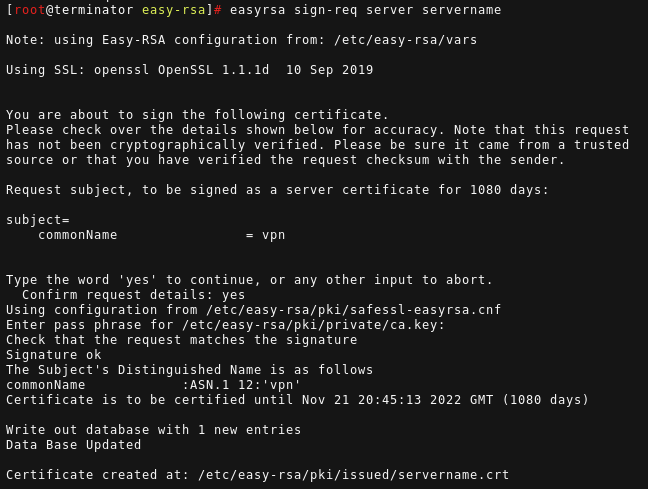
\includegraphics[width=1\textwidth]{resources/ca17.png}
                \caption{Firmamos como servidor la clave pública recepcionada.}
                \label{ca17}
            \end{figure}
        
            Hacemos posteriormente lo mismo con la clave del cliente \textit{terminator} en este caso, 
            pero en vez de firmar como servidor lo haremos, lógicamente, como cliente.
        
            \begin{figure}[htp]
                \centering
                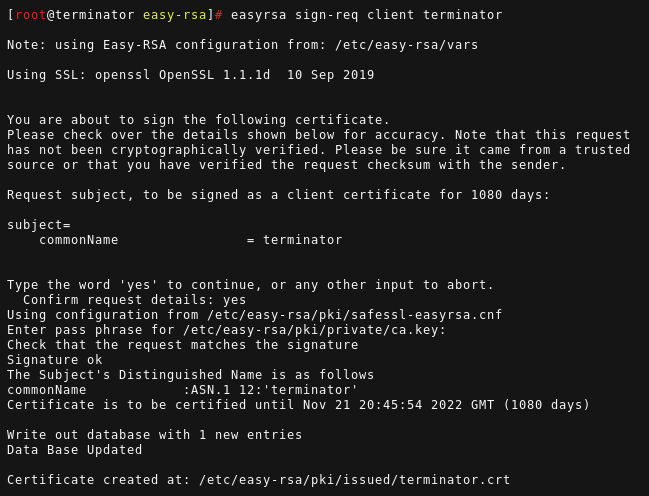
\includegraphics[width=1\textwidth]{resources/ca18.png}
                \caption{Firmamos como cliente la clave pública recepcionada de cliente.}
                \label{ca18}
            \end{figure}
        
            Entonces, observaremos en la ruta \textit{/etc/easy-rsa/pki/issued/} las claves firmadas.
        
            \begin{figure}[htp]
                \centering
                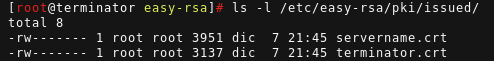
\includegraphics[width=1\textwidth]{resources/ca19.png}
                \caption{Certificados firmados en servidor CA.}
                \label{ca19}
            \end{figure}
        
            Enviamos estas claves a sus respectivos propietarios mediante el procotolo seguro SCP.
        
            \begin{figure}[htp]
                \centering
                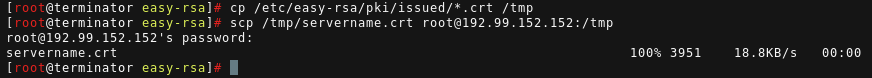
\includegraphics[width=1\textwidth]{resources/ca20.png}
                \caption{Enviamos los certificados firmados a sus respectivos propietarios.}
                \label{ca20}
            \end{figure}
        
            Para finalizar, simplemente debemos mover los certificados recibidos por sus propietarios
            a sus respectivas rutas.
        
            \begin{figure}[htp]
                \centering
                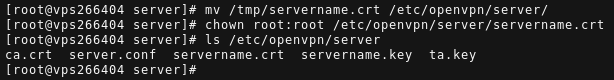
\includegraphics[width=1\textwidth]{resources/ca21.png}
                \caption{Movemos en el servidor el certificado firmado a \textit{/etc/openvpn/server/}.}
                \label{ca21}
            \end{figure}
        
            \begin{figure}[htp]
                \centering
                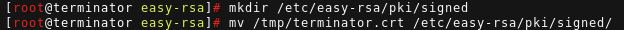
\includegraphics[width=1\textwidth]{resources/ca22.png}
                \caption{Movemos en el cliente el certificado firmado a \textit{/etc/easy-rsa/pki/signed}.}
                \label{ca22}
            \end{figure}

    \newpage
    \newpage
    \newpage
    \subsection{Configuración del servidor}

        Una vez llegados a este punto, en el lado del servidor VPN deberemos tener los siguientes
        4 ficheros en la ruta \textit{/etc/openvpn/server/}:

        \begin{itemize}
            \item ca.crt
            \item servername.crt
            \item servername.key
            \item ta.key
        \end{itemize}

        \subsubsection{Configuración básica de enrutamiento en la capa de red (capa 3 en el modelo
        OSI)}

            Lo primero que debemos hacer es obtener un fichero de configuración (\textit{server.conf}) que define
            los diferentes parámetros y, como su nombre indica, configuraciones del servidor OpenVPN. Podemos crear 
            uno desde cero manualmente o bien partir de uno de los ficheros de ejemplo para editarlo y adecuarlo a 
            nuestras necesidades.
        
            \begin{figure}[htp]
                \centering
                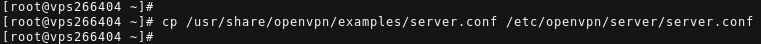
\includegraphics[width=1\textwidth]{resources/openvpn04.png}
                \caption{Copia de fichero de configuración de ejemplo en el directorio del servidor.}
                \label{}
            \end{figure}
        
            En cuanto a la configuración destacamos las líneas \textit{dh none} y \textit{ecdh-curve secp521r1}, que
            indica al servidor que estamos utilizando TLS con curvas elípticas. El archivo de parámetros DH no será
            necesario por el mismo motivo.
        
            \begin{figure}[htp]
                \centering
                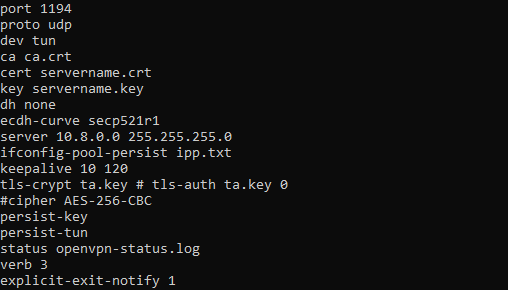
\includegraphics[width=1\textwidth]{resources/openvpn05.png}
                \caption{Configuración base del servidor OpenVPN.}
                \label{}
            \end{figure}    
    
    
        \subsubsection{Hardening del servidor}

            Para mejorar la seguridad y <<endurecer>> y robustecer el servidor podemos utilizar configuraciones 
            adicionales que incluye: limitar el servidor para usar un método de cifrado y autenticación seguro y 
            (opcionalmente) limitar el conjunto de cifrados TLS habilitados a los cifrados más nuevos. Para
            ello podemos añadir las siguientes líneas a nuestro archivo de configuración:
        
            \begin{figure}[htp]
                \centering
                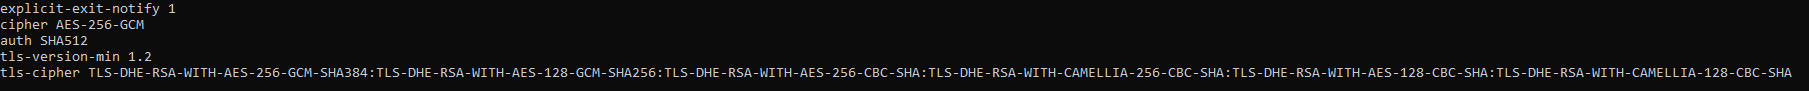
\includegraphics[width=1\textwidth]{resources/openvpn06.png}
                \caption{Líneas para mejorar la seguridad del servidor robusteciendo su cifrado.}
                \label{}
            \end{figure} 
        
            Pero, debido a que estamos en una versión superior a \textit{OpenVPN 2.4} la seguridad utilizada
            por defecto es suficiente para tener un alto nivel de seguridad, utilizando el cifrado 
            \textit{AES-256-GCM}\footnote{
                GCM (Galois Counter Mode) es un modo de operación para cifrados de bloques criptográficos de
                claves simétricas. GCM es ideal para proteger paquetes de datos porque tiene baja latencia 
                y una sobrecarga de operación mínima.
            }
            por defecto.
        
            Con el objetivo de mantener un nivel de robustez elevado, una configuración esencial, siempre que
            sea posible, es utilizar el protocolo UDP en nuestro servidor.
            TCP sobre TCP es una mala idea. % TODO http://sites.inka.de/bigred/devel/tcp-tcp.html
            Por ello se recomienda usar OpenVPN sobre UDP.
    
        \subsubsection{Posible desviación de puertos y protocolos}
        
            Algunas redes pueden no permitir conexiones OpenVPN en el puerto y/o protocolo predeterminados. 
            Una estrategia para eludir esto es imitar el tráfico HTTPS que probablemente no esté obstruido.
            
            Para lograr ello símplemente deberíamos configurar el puerto como 443 (usado por HTTPS) y 
            el protocolo TCP, en sus parámetros \textit{port 443} y \textit{proto tcp} en el archivo de
            configuración con el que estamos tratando (\textit{/etc/openvpn/server/server.conf}). Pero teniendo
            en cuenta los parámetros de hardening no es recomendable realizar esta acción a no ser que sea
            estrictamente necesario.
            
    \subsection{Elevación del servidor}

        Una vez se haya configurado el servidor podremos levantar el servicio para probar su correcta
        configuración. Como podemos observar en la figura \ref{openvpn08} la configuración ha funcionando
        correctamente y el servidor se ha levantado sin problemas.

        \begin{figure}[htp]
            \centering
            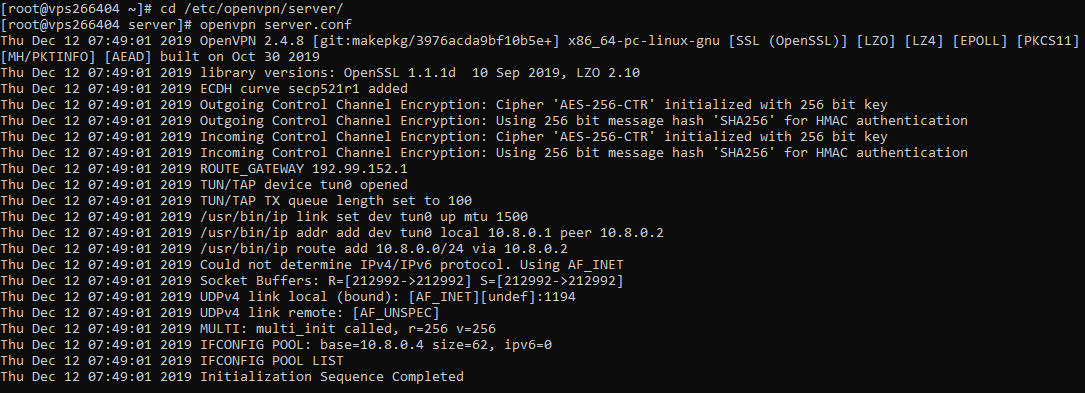
\includegraphics[width=1\textwidth]{resources/openvpn08.png}
            \caption{Log de inicio del servidor OpenVPN.}
            \label{openvpn08}
        \end{figure}   

        Para estar aún más seguros de ello podemos comprobar mediante \textit{ifconfig}. observaremos
        las dos tarjetas de red base que tenía el servidor, como vienen a ser \textit{lo}\footnote{
            La interfaz de bucle invertido o \textit{Loopback, lo}; no representa ningún hardware 
            real, pero existe para que las aplicaciones que se ejecutan en el equipo siempre puedan
            conectar a esta tarjeta ficticia sin necesidad de hardware funcional o configuración de 
            red hablitada en otras interfaces. Podemos decir que es la que habilita \textit{localhost} o
            su dirección local \textit{127.0.0.1}.
        }
        y \textit{etho}, siendo esta segunda la interfaz principal (\textit{0}) de la tarjeta de red 
        \textit{Ethernet}, con información de ésta como su dirección física (MAC) y su configuración de 
        red IPv4 e IPv6.
        
        Pero junto a ellas podemos observar una nueva interfaz denominada \textit{tun0}, que corresponde 
        a la interfaz creada por \textit{TUN}, tal y como vimos en puntos anteriores. Del mismo modo que
        \textit{lo}, o en especial \textit{eth0} observamos la configuración de direcciones IPv4 e IPv6;
        siendo éstas las direcciones configuradas previamente la configuración del 
        servidor OpenVPN en el parámetro \textit{server}, con la red \textit{10.8.0.0/24} ó
        \textit{10.8.0.0 255.255.255.0} (véase fichero de configuración del servidor 
        \textit{/etc/openvpn/server/server.conf}).

        \begin{figure}[htp]
            \centering
            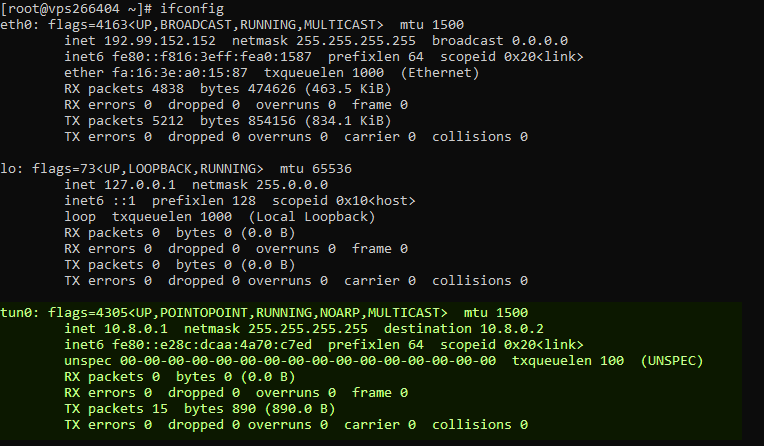
\includegraphics[width=1\textwidth]{resources/openvpn09.png}
            \caption{Demostración de funcionamiento de tarjetas de red con servidor OpenVPN levantado 
            (tun0 levantado).}
            \label{}
        \end{figure}   

        Debido a que es el primer equipo de la red (natural, siendo su servidor)
        \textit{10.8.0.0} y de acuerdo a su máscara de red \textit{255.255.255.0}, el DHCP 
        propio de OpenVPN ha asignado a éste la dirección \textit{10.8.0.1}.
        
\section{Implementación de clientes, método \textit{.conf}}

    \subsection{Cliente Arch Linux, GNU/Linux x86\_64}

        Una vez tenemos nuestro servidor funcional y operativo, es el momento de asignarle el primer 
        cliente VPN. Éste será el ya configurado \textit{terminador}. Recordemos que \textit{terminator}
        es un servidor físico Arch Linux que hará de proveedor de algunos servicios en la red al 
        resto de clientes. Pero aún tratándose de un servidor de cara a la configuración de
        esta estructura es cliente de este servicio.

        Lo primero que haremos es trasladar los archivos \textit{ca.crt}, \textit{terminator.crt}
        y \textit{terminator.key} al directorio \textit{/etc/openvpn/client/}, del mismo modo que 
        con el servidor. También copiaremos (del fichero de pruebas \textit{/usr/share/openvpn/examples/client.conf})
        o bien lo creamos manualmente.

        \begin{figure}[htp]
            \centering
            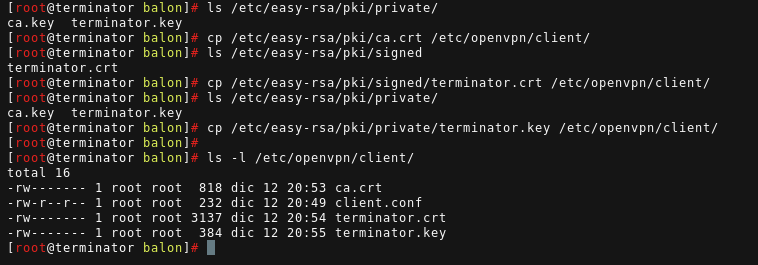
\includegraphics[width=1\textwidth]{resources/openvpn10.png}
            \caption{Obtención de ficheros necesarios para configuración de cliente.}
            \label{}
        \end{figure}   

        La configuración del fichero \textit{client.conf} constará de los siguientes elementos,
        expuestos en la figura \ref{openvpn11}. La configuración del cliente debe concordar,
        evidentemente con la del servidor en protocolo y seguridad; si este segundo no estuviera
        bien definido no podríamos autenticar el cliente correctamente. A destacar los parámetros
        \textit{ca}, \textit{cert} y \textit{key} que deberán apuntar a los ficheros que hemos
        traído en los puntos anteriores. Finalmente es necesario indicar la dirección del servidor
        en el parámetro \textit{remote}, de forma que el cliente apunte a éste\footnote{
            Si en lugar de la dirección IP quisiéramos indicar un nombre de dominio debemos
            cercionarnos que el servidor DNS esté adecuadamente configurado para que no se 
            den errores en la traducción de nombres.
        }. El puerto, lógicamente será el configurado en el servidor.

        \begin{figure}[htp]
            \centering
            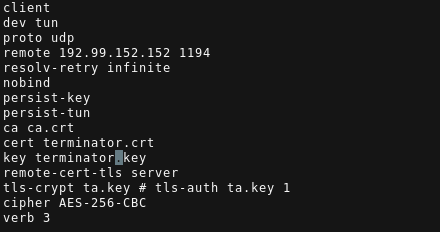
\includegraphics[width=1\textwidth]{resources/openvpn11.png}
            \caption{Fichero de configuración de cliente OpenVPN.}
            \label{openvpn11}
        \end{figure}   

        Del mismo modo que el servidor, si queremos iniciar el cliente llegados a este punto 
        para probar que la configuración esté correcta, se realizará mediante el comando propio
        \textit{openvpn} seguido del fichero de configuración.

        Como vemos en la figura \ref{openvpn12}, algo no ha ido bien. El cliente OpenVPN no 
        ha sido levantado y en el log de inicio podemos ver una descripción del error que lo ha 
        impedido: \textit{<<--tls-crypt fails with ta.key: No such file or directory>>}. El 
        error está claro, no tenemos el fichero \textit{ta.key} del servidor para la configuración
        del cifrado TLS entre el cliente y el servidor.

        \begin{figure}[htp]
            \centering
            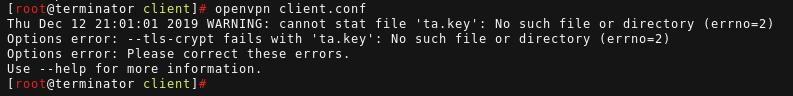
\includegraphics[width=1\textwidth]{resources/openvpn12.png}
            \caption{Prueba fallida de inicio de cliente OpenVPN.}
            \label{openvpn12}
        \end{figure}   

        Para solucionar esto, nos traemos al cliente una copia del servidor mediante el protocolo
        SCP. Y éste lo enviamos al directorio con el resto de ficheros.

        \begin{figure}[htp]
            \centering
            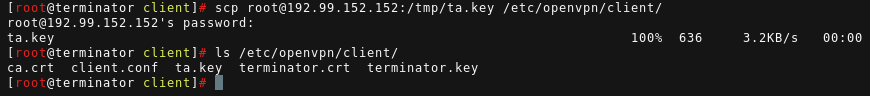
\includegraphics[width=1\textwidth]{resources/openvpn13.png}
            \caption{Obtención por parte del cliente de \textit{ta.key} del servidor.}
            \label{}
        \end{figure}   

        De esta forma, podemos volver a probar la configuración iniciando el servicio, que como
        observamos en la figura \ref{openvpn14}, todo ha ido correctamente y el servicio se ha 
        iniciado. \textbf{Tenemos cliente activo en la red VPN}.

        \begin{figure}[htp]
            \centering
            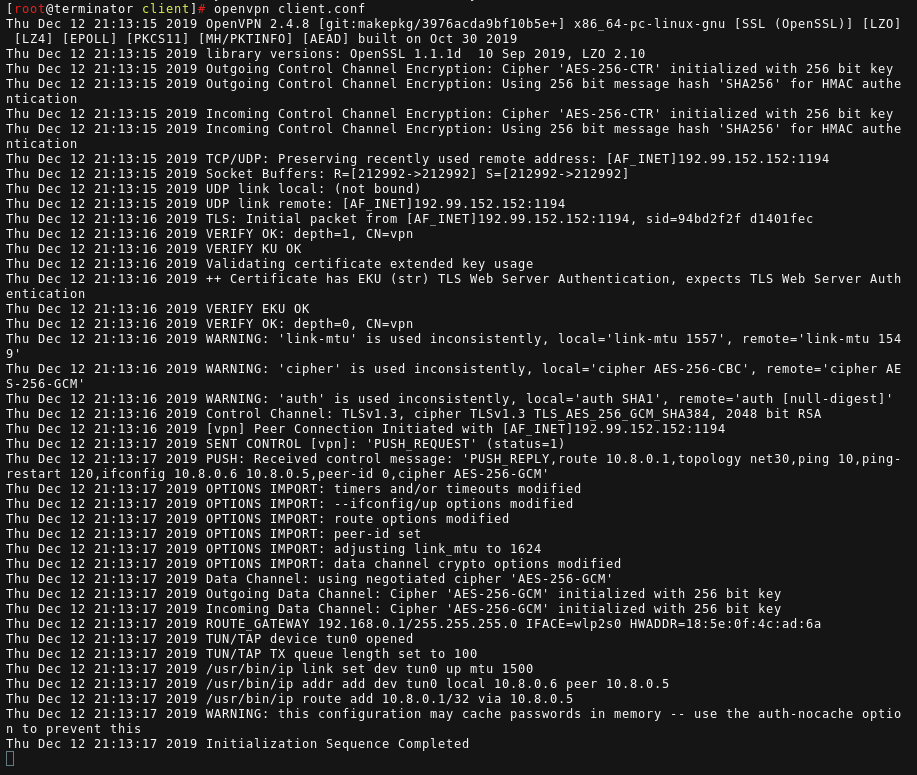
\includegraphics[width=1\textwidth]{resources/openvpn14.png}
            \caption{Log de inicio satisfactorio de cliente OpenVPN.}
            \label{openvpn14}
        \end{figure}   

        Si nos dirigimos a la configuración de red de nuevo, tal y como hicimos con el servidor
        pero en este caso en el cliente observaremos su configuración de redes propia:

        \begin{itemize}
            \item \textit{enp1s0f1}. Tarjeta de red Ethernet.
            \item \textit{lo}. Tarjeta de red \textit{Loopback}.
            \item \textit{wlp2s0}. Tarjeta de red Wi-Fi.
            \item \textit{tun0}. Y finalmente, el túnel TUN creado para el cliente. Sin entrar 
            a explicar todo, pues funciona de la misma forma que en el servidor, podemos ver la
            configuración de túnel \textit{10.8.0.6/24}; dirección asignada por el DHCP propio.
        \end{itemize}

        \begin{figure}[htp]
            \centering
            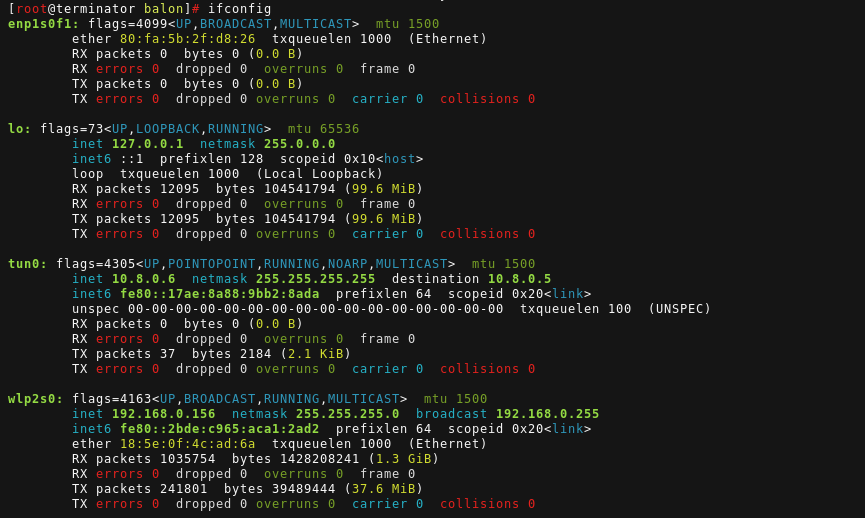
\includegraphics[width=1\textwidth]{resources/openvpn15.png}
            \caption{Configuración de red del cliente OpenVPN. A destacar la creación de \textit{tun0}.}
            \label{}
        \end{figure}   

        La prueba más elemental que haremos ahora será probar la comunicación entre ambos mediante
        \textit{ping}. Evidentemente utilizaremos las direcciones de la red VPN. Esto lo podemos
        observar en las imágenes \ref{fig:openvpn1617}.

        \begin{figure}[htp]
        \centering
            \begin{subfigure}[b]{1\linewidth}
            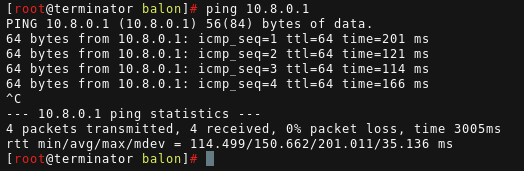
\includegraphics[width=1\textwidth]{resources/openvpn16.png}
            \caption{Ping de cliente (\textit{10.8.0.6}) a servidor (\textit{10.8.0.1}).}
            \end{subfigure}

            \begin{subfigure}[b]{1\linewidth}
            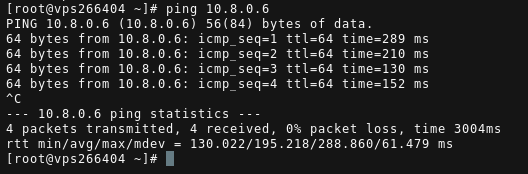
\includegraphics[width=1\textwidth]{resources/openvpn17.png}
            \caption{Ping de servidor (\textit{10.8.0.1}) a cliente (\textit{10.8.0.6}).}
            \end{subfigure}
        \caption{Comunicación entre cliente y servidor.}
        \label{fig:openvpn1617}
        \end{figure}

    \newpage
    \newpage
    \subsection{Cliente Raspberry Pi 4 (Raspbian, GNU/Linux ARM)}

        La instalación de OpenVPN como cliente en una máquina Raspberry Pi en su modelo <<4>>
        es similar a la creación de cualquier cliente Linux. El primer paso es el que de ahora 
        en adelante veremos como común y típico; la creación de los ficheros de cliente en el
        servidor CA y su posterior recepción por parte de éste último (figura \ref{fig:raspy0102}).

        \begin{figure}[htp]
        \centering
            \begin{subfigure}[b]{1\linewidth}
            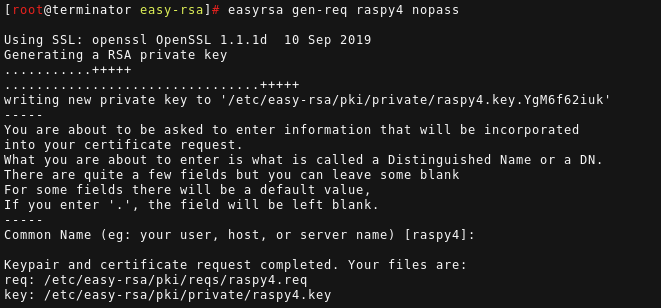
\includegraphics[width=1\textwidth]{resources/raspy01.png}
            \caption{Generación de certificados para cliente \textit{raspy4}.}
            \end{subfigure}

            \begin{subfigure}[b]{1\linewidth}
            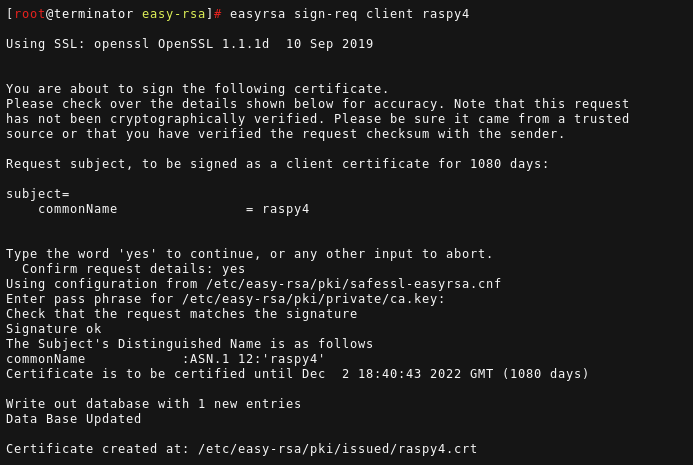
\includegraphics[width=1\textwidth]{resources/raspy02.png}
            \caption{Firma de certificados de \textit{raspy4} por \textit{CA}.}
            \end{subfigure}
        \caption{Generación y firma de certificados.}
        \label{fig:raspy0102}
        \end{figure}

        El siguiente paso lo podemos observar en la figura \ref{fig:raspy0306}, consistente en 
        la unificación y envío de los archivos necesarios al cliente. Estos, como de costumbre
        en este documento son los archivos \textit{ca.crt}, \textit{client.conf}, \textit{client.crt}
        y \textit{Client.key} y \textit{ta.key}.

        \begin{figure}[htp]
        \centering
            \begin{subfigure}[b]{0.8\linewidth}
            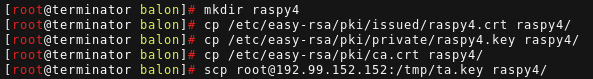
\includegraphics[width=1\textwidth]{resources/raspy03.png}
            \caption{Preparación de archivos de cliente \textit{raspy4}.}
            \end{subfigure}

            \begin{subfigure}[b]{1\linewidth}
            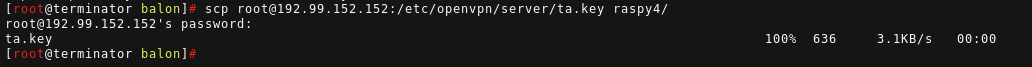
\includegraphics[width=1\textwidth]{resources/raspy04.png}
            \caption{Descarga del servidor OpenVPN \textit{ta.key}.}
            \end{subfigure}
                
            \begin{subfigure}[b]{0.6\linewidth}
            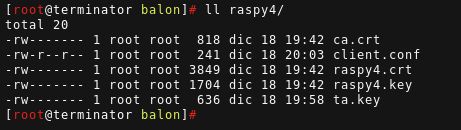
\includegraphics[width=1\textwidth]{resources/raspy05.png}
            \caption{Archivos de cliente necesarios agrupados.}
            \end{subfigure}

            \begin{subfigure}[b]{0.6\linewidth}
            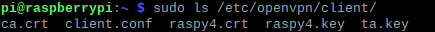
\includegraphics[width=1\textwidth]{resources/raspy06.png}
            \caption{Archivos en cliente.}
            \end{subfigure}
        \caption{Intercambio de archivos en cliente.}
        \label{fig:raspy0306}
        \end{figure}

        Posteriormente únicamente queda levantar el servicio en el lado del cliente y observar la
        correcta recepción de la configuración por parte del servidor. Podemos ver en la figura 
        \ref{fig:raspy07} el log de puesta en marcha del servicio OpenVPN elevado.

        \begin{figure}[htp]
        \centering
        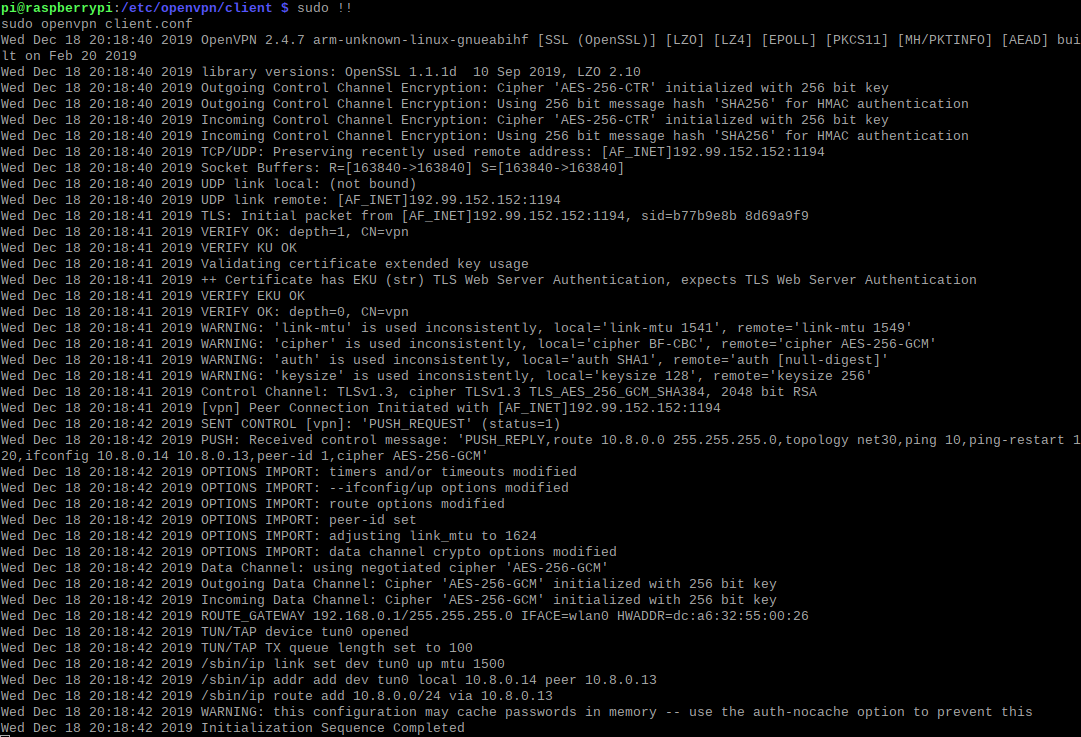
\includegraphics[width=1\textwidth]{resources/raspy07.png}
        \caption{Log de puesta en marcha de OpenVPN en \textit{raspy4}.}
        \label{fig:raspy07}
        \end{figure}  

        Lo que dará como resultado la nueva interfaz \textit{TUN} que observamos en la configuración
        de redes del dispositivo \textit{Raspberry Pi 4}. Podemos observarlo en la figura \ref{fig:raspy08},
        habiendo recibido la dirección IP \textit{10.8.0.14}. Y finalizamos la configuración probando la 
        conectividad con el servidor (figura \ref{fig:raspy09}).

        \begin{figure}[htp]
            \centering
            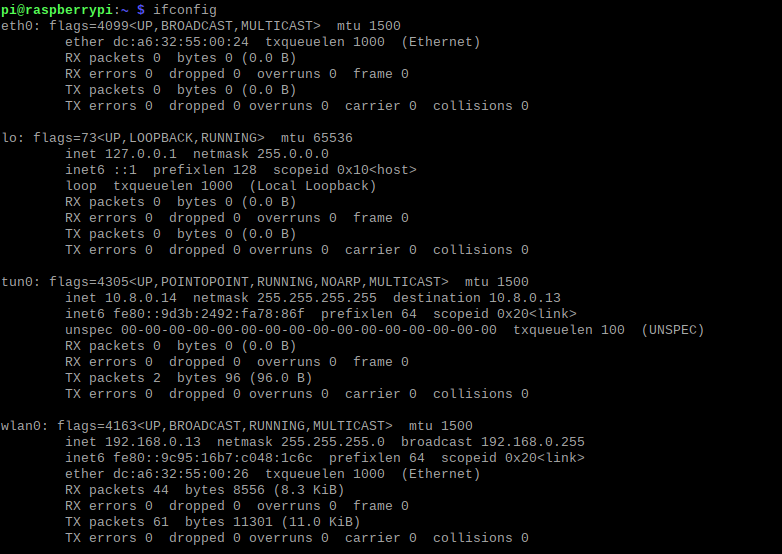
\includegraphics[width=1\textwidth]{resources/raspy08.png}
            \caption{Configuración de redes de \textit{raspy4}.}
            \label{fig:raspy08}
        \end{figure}  

        \begin{figure}[htp]
            \centering
            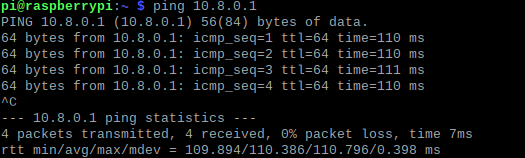
\includegraphics[width=0.8\textwidth]{resources/raspy09.png}
            \caption{Prueba de conectividad con servidor OpenVPN a través del túnel VPN creado.}
            \label{fig:raspy09}
        \end{figure}  

    \subsection{Cliente Microsoft Windows 10}

        No entraremos en la descarga e instalación de OpenVPN en el sistema operativo de
        Microsoft debido a que no se trata de hacer un tutorial de instalación sino una 
        documentación de la propia infraestructura. Simplemente añadiremos la configuración
        necesaria para su funcionamiento.

        La generción y firma de certificados la podemos ver en la figura \ref{fig:windows0102}.

        \begin{figure}[htp]
        \centering
            \begin{subfigure}[b]{1\linewidth}
            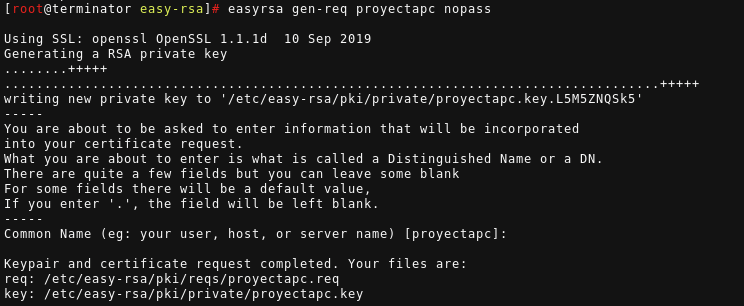
\includegraphics[width=1\textwidth]{resources/windows01.png}
            \caption{Generación de certificados para cliente \textit{proyectapc}.}
            \end{subfigure}

            \begin{subfigure}[b]{1\linewidth}
            \includegraphics[width=1\textwidth]{resources/windows02.png}
            \caption{Firma de certificados de \textit{proyectapc} por \textit{CA}.}
            \end{subfigure}
        \caption{Generación y firma de certificados.}
        \label{fig:windows0102}
        \end{figure}

        Posteriormente obtendremos los archivos necesarios y los copiamos en el cliente. Podemos
        reutilizar el archivo \textit{conf} del cliente \textit{terminator}, ya configurado, de forma
        que no tendremos que generarlo de nuevo y la configuración sería mínima.

        \begin{figure}[htp]
        \centering
            \begin{subfigure}[b]{1\linewidth}
            \includegraphics[width=1\textwidth]{resources/windows03.png}
            \caption{Unificamos los archivos necesarios para el cliente OpenVPN.}
            \end{subfigure}

            \begin{subfigure}[b]{0.8\linewidth}
            \includegraphics[width=1\textwidth]{resources/windows04.png}
            \caption{Copiamos la configuración del cliente \textit{terminator} para reutilizar
            código en \textit{proyectapc}.}
            \end{subfigure}

            \begin{subfigure}[b]{0.7\linewidth}
            \includegraphics[width=1\textwidth]{resources/windows05.png}
            \caption{Configuración \textit{client.conf} de \textit{proyectapc}.}
            \end{subfigure}
        \caption{Intercambio de archivos en cliente.}
        \label{fig:windows0305}
        \end{figure}

        Para algunos clientes, como Microsoft Windows o Android podemos generar el archivo rápido
        \textit{ovpn}. Éste guarda en sí mismo todos los archivos anteriores y facilita aún más, si 
        cabe, la configuración. Podremos utilizar indistintivamente el archivo \textit{conf} o 
        \textit{ovpn} sin ningún problema, pues es prácticamente similar.

        En el caso de la distribución utilizada por el servidor CA se encuentra en el repositorio 
        AUR, por lo que utilizaremos la herramienta \textit{aurman} para instalar el script 
        denominado \textit{ovpngen}. Esto lo podemos observar en la figura \ref{fig:windows06}.

        \begin{figure}[htp]
            \centering
            \includegraphics[width=0.7\textwidth]{resources/windows06.png}
            \caption{Instalación de \textit{ovpngen} desde \textit{aurman}.}
            \label{fig:windows06}
        \end{figure}  

        La generación con \textit{ovpngen} es sencilla, simplemente le pasaremos como parámetros las
        rutas de los distintos archivos que componen el conjunto de la configuración del cliente,
        y en la ruta y con el nombre elegido será generado el archivo \textit{ovpn} (figura \ref{fig:windows07}).

        \begin{figure}[htp]
            \centering
            \includegraphics[width=0.9\textwidth]{resources/windows07.png}
            \caption{Generación de \textit{ovpn}.}
            \label{fig:windows07}
        \end{figure}  

        Una vez finalizado, enviaremos los archivos necesarios al sistema cliente, que en este caso
        es un Microsoft Windows 10. Podemos observar la prueba en la figura \ref{fig:windows08}.

        \begin{figure}[htp]
            \centering
            \includegraphics[width=0.8\textwidth]{resources/windows08.png}
            \caption{Archivos \textit{proyectapc} en cliente.}
            \label{fig:windows08}
        \end{figure}  

        Utilizando el software OpenVPN para Microsoft Windows, simplemente le indicaremos dónde
        se encuentran los ficheros de configuración. Deberemos indicarle también si queremos 
        utilizar el archivo \textit{conf} o el archivo \textit{ovpn} que generamos previamente
        (\ref{fig:windows09}).

        \begin{figure}[htp]
            \centering
            \includegraphics[width=0.6\textwidth]{resources/windows09.png}
            \caption{Configuración de OpenVPN GUI.}
            \label{fig:windows09}
        \end{figure}  

        Y simplemente lanzamos el cliente OpenVPN (\ref{fig:windows10}).

        \begin{figure}[htp]
            \centering
            \includegraphics[width=0.6\textwidth]{resources/windows10.png}
            \caption{Conexión con servidor OpenVPN.}
            \label{fig:windows10}
        \end{figure}  

        \newpage
        Finalmente y como hemos hecho en el resto de clientes, comprobamos la correcta inicialización
        y configuración del cliente. Observamos primero la configuración de red del cliente \textit{proyectapc}
        en la figura \ref{fig:windows11}.
        En la misma observamos cómo el servidor DHCP del servidor OpenVPN nos ofrece la dirección 
        \textit{10.8.0.6}\footnote{
            El documento se ha desarrollado en diferentes días, por lo que es posible que la dirección
            IP dada por el servidor en un momento concreto coincida con la de otro cliente, como se ha 
            dado el caso. Aunque coincidan en la documentación, no sería posible así en la red.
        }.

        \begin{figure}[htp]
            \centering
            \includegraphics[width=1\textwidth]{resources/windows11.png}
            \caption{Comprobación de IP obtenida por DHCP.}
            \label{fig:windows11}
        \end{figure}  

        Probamos además la comunicación con el servidor (figura \ref{fig:windows12}).

        \begin{figure}[htp]
            \centering
            \includegraphics[width=1\textwidth]{resources/windows12.png}
            \caption{Comprobación de ping al servidor mediante el túnel creado.}
            \label{fig:windows12}
        \end{figure}  

\section{Diseño de redes y subredes cliente-servidor}

    \subsection{Comunicación entre clientes}

        Ya sabemos que al conectarnos a la red privada virtual el servidor asigna a cada 
        clientes una dirección IP perteneciente a una subred predefinida (\textit{10.8.0.0/24}
        en este caso concreto) mediante el protocolo DHCP). Sin embargo, y a pesar de que 
        todos los clientes de una misma VPN poseen direcciones IP de una misma subred, por 
        defecto no existe conectividad entre los mismos. Esto es una medida de seguridad
        que implementa OpenVPN que permite la no exposición de estos nodos de la red a no
        ser que indiquemos lo contrario. 

        La solución a esto es muy sencilla. Simplemente añadimos \textit{client-to-client}
        en el archivo de configuración del servidor OpenVPN. Esto indicará al servidor
        la habilitación de conectividad entre clientes.

        \begin{figure}[htp]
            \centering
            \includegraphics[width=0.5\textwidth]{resources/configs01.png}
            \caption{Añadiendo la línea \textit{client-to-client} en \textit{/etc/openvpn/server/server.conf}.}
            \label{}
        \end{figure}  

        Para prueba, realizamos ping entre el cliente \textit{terminator} y el cliente \textit{proyectapc}.

        \begin{figure}[htp]
            \centering
            \includegraphics[width=0.8\textwidth]{resources/configs02.png}
            \caption{Ping entre clientes \textit{terminator} y \textit{proyectapc}.}
            \label{}
        \end{figure}  
    
        De esta forma tenemos una emulación perfecta de red local, permitiendo utilizar cualquier
        protocolo para interacturar entre ellos. Por ejemplo, utilizaremos el protocolo RDP para
        controlar remota y gráficamente el cliente Windows desde el cliente GNU/Linux desde una
        red completamente diferente pero ambos en la misma red VPN que hemos levantado (figura \ref{fig:configs03}).
    
        \begin{figure}[htp]
            \centering
            \includegraphics[width=1\textwidth]{resources/configs03.png}
            \caption{Control remoto RDP de cliente \textit{proyectapc} desde \textit{terminator}.}
            \label{fig:configs03}
        \end{figure} 
    
        \newpage

    \subsection{Elevando múltiples instancias de OpenVPN en diferentes puertos del servidor físico}

        Podemos, utilizando las mismas claves criptográficas levantar tantos servidores OpenVPN en tantos
        puertos de la máquina física servidora como queramos (dentro de las limitaciones de puertos y de las
        características de nuestra máquina).

        Para ello simplemente debemos crear un nuevo archivo de configuración de servidor, o bien
        copiar el ya existente con el objetivo de realizar los cambios oportunos, que generalmente 
        son mínimos. En este caso hemos realizado 3 cambios (figura \ref{fig:configs04}):

        \begin{figure}[htp]
            \centering
            \includegraphics[width=0.7\textwidth]{resources/configs04.png}
            \caption{Copia realizada a fichero de configuración.}
            \label{fig:configs04}
        \end{figure} 

        \begin{itemize}
            \item El puerto utilizado 1194 pasa a ser el 443.
            \item El protocolo pasa de UDP a TCP.
            \item La subred pasa de 10.8.0.0/24 a 10.8.1.0/24.
        \end{itemize}

        Finalmente vemos en nuestro servidor 2 interfaces TUN denominadas \textit{tun0} y \textit{tun1},
        respectivamente, haciendo de servidores de sus respectivas subredes VPN (figura \ref{fig:configs05}).

        \begin{figure}[htp]
            \centering
            \includegraphics[width=1\textwidth]{resources/configs05.png}
            \caption{Configuración de red de servidor.}
            \label{fig:configs05}
        \end{figure} 

        \newpage
    \subsection{Múltiples redes en clientes}

        Del mismo modo, un cliente puede encontrarse en diferentes redes VPN sin necesidad de estar
        estas unidas entre sí ni tener nada que ver. 

        \begin{figure}[htp]
            \centering
            \includegraphics[width=1\textwidth]{resources/configs06.png}
            \caption{Configuración de red de cliente con múltiples clientes VPN.}
            \label{fig:configs05}
        \end{figure} 

\section{Resumen de securización y hardening de la red VPN}

    Para finalizar, documentaremos el proceso de securización y hardening de la red VPN. Pero
    no habrá nada nuevo que no se haya tratado ya. Todos los puntos que serán expuestos en este 
    apartado no serán más que recuerdos de lo que ya se ha hecho. 

    El hardening se ha realizado durante todo el proceso, ya que la seguridad de la red no es 
    un producto estático, sino un proceso dinámico que evoluciona y cambia.

    Por ello recordamos:
    
    \begin{itemize}
        \item El uso de protocolos seguros para la transferencia y comunicación entre equipos
        durante la edificación de la red VPN, tales como SCP y SSH, respectivamente. La razón 
        es sencilla: evitar escuchas no deseadas o sniffer que puedan robar nuestras claves
        para suplantar en el futuro a un cliente de nuestra red o tener acceso a ella. 
        Es importante realizar todas las operaciones mediante métodos certificados y seguros, 
        con una capa criptográfica como mínimo.
        \item TSL para las comunicaciones VPN.
        \item Criptografía de curva elíptica, para hacer más cómodo y seguro el intercambio de
        información de sesión.
        \item Del mismo modo, el uso de Hash-based Message Authentication Code (HMAC) key para 
        la autenticación de clientes.
        \item Hemos realizado además el proceso de hardening de la configuración del servidor,
        para robustecer el mismo ante distintos tipos de ataques.
        \item No habilitamos compresión para evitar ataques vectoriales.
        \item TCP sobre UDP para mayor seguridad siempre que sea posible.
    \end{itemize}
    
% BIBLIOGRAFÍA Y REFERENCIAS
\newpage
\begin{thebibliography}{X}
    \bibitem{} OpenVPN en Arch Wiki - wiki.archlinux.org/index.php/OpenVPN
    \bibitem{} Easy-RSA en Arch Wiki - wiki.archlinux.org/index.php/Easy-RSA
    \bibitem{} TUN/TAP Tunnels - rrendec.mindbit.ro/post/tun-tap-tunnels/
    \bibitem{} TUN/TAP in Linux Documentation - github.com/torvalds/linux/blob/master/Documentation/networking/tuntap.txt
    \bibitem{} Secure Computing in PKI - secure-computing.net/openvpn/howto.php\#pki
    \bibitem{} James Yonan Interview - linuxsecurity.com/features/features/openvpn-an-introduction-and-interview-with-founder-james-yonan
    \bibitem{} Repositorio del proyecto OpenVPN en Github - github.com/OpenVPN/openvpn
    \bibitem{} Why TCP Over TCP Is A Bad Idea - sites.inka.de/bigred/devel/tcp-tcp.html
    \bibitem{} Hardening Openvpn for DEFCON - agwa.name/blog/post/hardening\_openvpn\_for\_def\_con
\end{thebibliography}

\end{document}